%!TEX root = ../../secondYearReport.tex


\paragraph{Work package 1 progress}

\subparagraph{Software architecture design and evaluation of available open-source software pertinent to the scope of the project. (T1.1)}

The explicit goal of T1.1 is for the consortium to agree on a specific software architecture with associated software tools whose specifications, dependencies and interconnections meet the requirements and needs for achieving the goals of the project.  To this end, the consortium met on 5th June 2013 at UPMC to discuss and agree on software interfaces, modules and architectures. The main outcomes from this meeting were: 
\begin{itemize}
\item IIT to develop plugins for Gazebo to interface with YARP. Gazebo chosen to be a replacement physics core for the iCubsim (see T1.2). 
\item UPMC to develop software using Orocos/XDE for whole body control and define generic interfaces for controllers, models, sensors, and actuation allowing for the communication of a C++ Orocos-based controller component with a robot using YARP or a YARP/Gazebo-based simulator.
\item  The consortium agreed on URDF as a unified modeling structure for defining and sharing descriptions of robots and human models. URDF is a standard XML format for representing the kinematic and dynamic description of a branched structure of articulated rigid bodies. 
\end{itemize}
The software architectural designs and specifications are to be documented as part of D1.2 and released at the end of year 2. 

\subparagraph{Simulator for whole-body motion with contacts (T1.2)}

The CoDyCo project requires a modular, component-based dynamics simulation software providing numerically stable, computationally efficient and physically consistent simulations of whole-body virtual human(oid) systems in contact with rigid or soft environments. To this end, in year one, a new iCub simulator has been released and documented as part of deliverable D1.1. In summary: 

\begin{itemize}
\item The previously existing iCub simulator needed an upgrade for more advanced applications including the multi-contact dynamics required for the CoDyCo project. The goal was to replace the physics core from ODE (Open Dynamics Engine) to one more suitable for articulated rigid body structures commonly used in robotics. To this end, Gazebo and XDE were chosen and evaluated as physics cores for the new iCub simulator. 

\item Partner UPMC led a survey of existing simulators for robotics\footnote{http://arxiv.org/abs/1402.7050}. In total 119 international robotics researchers responded to the survey.  

\item IIT contributed in CoDyCo with a joint activity with two other EU projects: Koroibot and WALK-MAN. The result of this collaboration is the development of a Gazebo plugin for exposing a YARP interface to the simulator. The plugin has been released with an open-source license and it is available on github (\url{https://github.com/robotology/gazebo_yarp_plugins}). At the moment of writing the current report, the plugin can be instantiated to control both COMAN (\url{https://github.com/EnricoMingo/iit-coman-ros-pkg}) and iCub (\url{https://github.com/robotology-playground/icub_gazebo}). This activity is related to a preliminary workshop publication \cite{Mingo2014}. 

\item Partner UPMC conducted a comparison between the XDE and Gazebo iCub simulators and a real iCub performing a leg free-falling task. In summary, in terms of predicted simulated outcomes, XDE and Gazebo are nearly numerically identical. However, both suffer with respect to accuracy, as the viscous friction models used are not able to accurately model the actual joint friction in the iCub. In conclusion, work in T1.4 (as well as WP3 and WP4) will need to address the issue of accurate friction modeling and estimation.

\item In order to provide a way to generate URDF models of digital mannequins independently from a specific simulator, JSI has developed a software for generating instances of a parametrized digital human (similar to the one present in XDE) as well as to edit the detailed parameters of an existing instance.  The new digital human URDF file generator is detailed in D1.1.
\end{itemize}

\subparagraph{Control library for flexible specification of task space dynamics of floating base manipulators. (T1.3)}

During the second year both IIT and UPMC contributed to the development of several software components for controlling the iCub whole-body behavior. The software has been structured around an abstraction layer called wholeBodyInterface, described in details within T3.2. This C++ abstraction layer is already used in a set of whole-body controllers implemented in simulink and available on github at the following address: \url{https://github.com/robotology/codyco/tree/master/src/simulink/controllers}. Within this context simulink is currently adopted as a fast designing tool for testing several controllers whose final implementation is foreseen in C++. Similarly, UPMC has started adopting the wholeBodyInterface within their own
controller framework based on XDE and ORCISI. Preliminary results are available here: \url{https://github.com/robotology/codyco/tree/master/src/tests}. 

%!TEX root = ../../secondYearReport.tex

\subparagraph{System dynamics estimation software. Extension to
environmental compliance estimation (T1.4)}

The goal of this task is to develop a software tool for on-line identification of whole-body dynamics, as well as the compliance of contacts established between the robot and the environment. 

\begin{itemize}
\item Within T1.4, IIT continued the activities started during the previous year, with specific focus on whole-body identification \cite{Traversaro2013, Traversaro2014}. In order to enhance the identification accuracy, an in-situ force/torque sensor calibration procedure was designed \cite{Traversaro2015b} (see Fig.~\ref{fig:validation}) and implemented in a software component\footnote{\url{https://github.com/robotology-playground/insitu-ft-calibration}.} which has been released with an open source license. Similarly, in order to enhance the torque estimation accuracy, IIT conducted a theoretical analysis that exploits embedded force/torque sensors. It has been proven \cite{Traversaro2015} that the inertial parameters estimated from embedded force/torque sensors can be successfully used for torque estimation.
\end{itemize}


\begin{figure}[h]
\vspace{0.5em}
\centering
{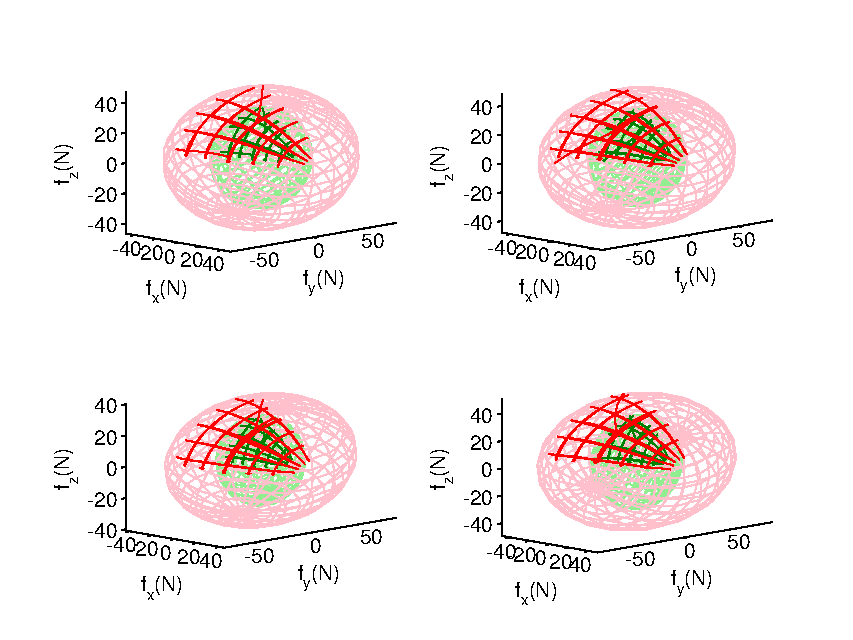
\includegraphics[width=0.65\textwidth]{images/leg_validation.pdf}}
\caption{The image shows the accuracy in calibrating the force/torque sensor with the procedure described in \cite{Traversaro2015b}. The four plots refer to four different experimental conditions (different values for the calibration weights). Ideally, perfectly calibrated data should lie on the surface of a three dimensional sphere. Dark green: force measurements obtained with the calibration matrix estimated using the proposed technique. Dark red: force measurements obtained with the calibration matrix provided with the sensor. Light red and light green surfaces: ellipsoids fitted to the measured forces. Qualitative calibration accuracy can be obtained by looking at the spherical symmetry of the fitted ellipsoids.}
\label{fig:validation}
\end{figure}

%!TEX root = ../../secondYearReport.tex

\subparagraph{Extension and enhancement of the iDyn library. (T1.5)}

Goal of this task is to provide a reliable software tool for on-line estimation of whole-body dynamics. Before CoDyCo, dynamic estimations on the iCub were relying on the iDyn software library\footnote{\url{https://github.com/robotology/icub-main/tree/master/src/libraries/iDyn}.}, designed for  fixed-base robots. Within the first year of CoDyCo, iDynTree\footnote{{\url{https://github.com/robotology/codyco/tree/master/src/libraries/iDynTree}}.} was released in response to the need of representing floating base structures. During the second year of the project, we investigated on the problem of extending iDynTree to the case of multiple redundant sensors. The investigation resulted in an experimental software library\footnote{\url{https://github.com/iron76/bnt_time_varying}.} currently implemented in \textsc{Matlab}. The software performs maximum-a-posteriori dynamic estimation fusing multiple sensors such as gyroscopes, linear accelerometers, embedded force-torque sensors and encoders. Computational efficiency is obtained by exploiting the sparsity of the underlying problem \cite{Nori2015} (see Fig.~\ref{fig:varTimeComplete}). Estimation accuracy is obtained by a modified version of the expectation maximisation algorithm \cite{Nori2015b} (see Fig.~\ref{fig:extForceEstimation}). 

\begin{figure}
  \centering 
	  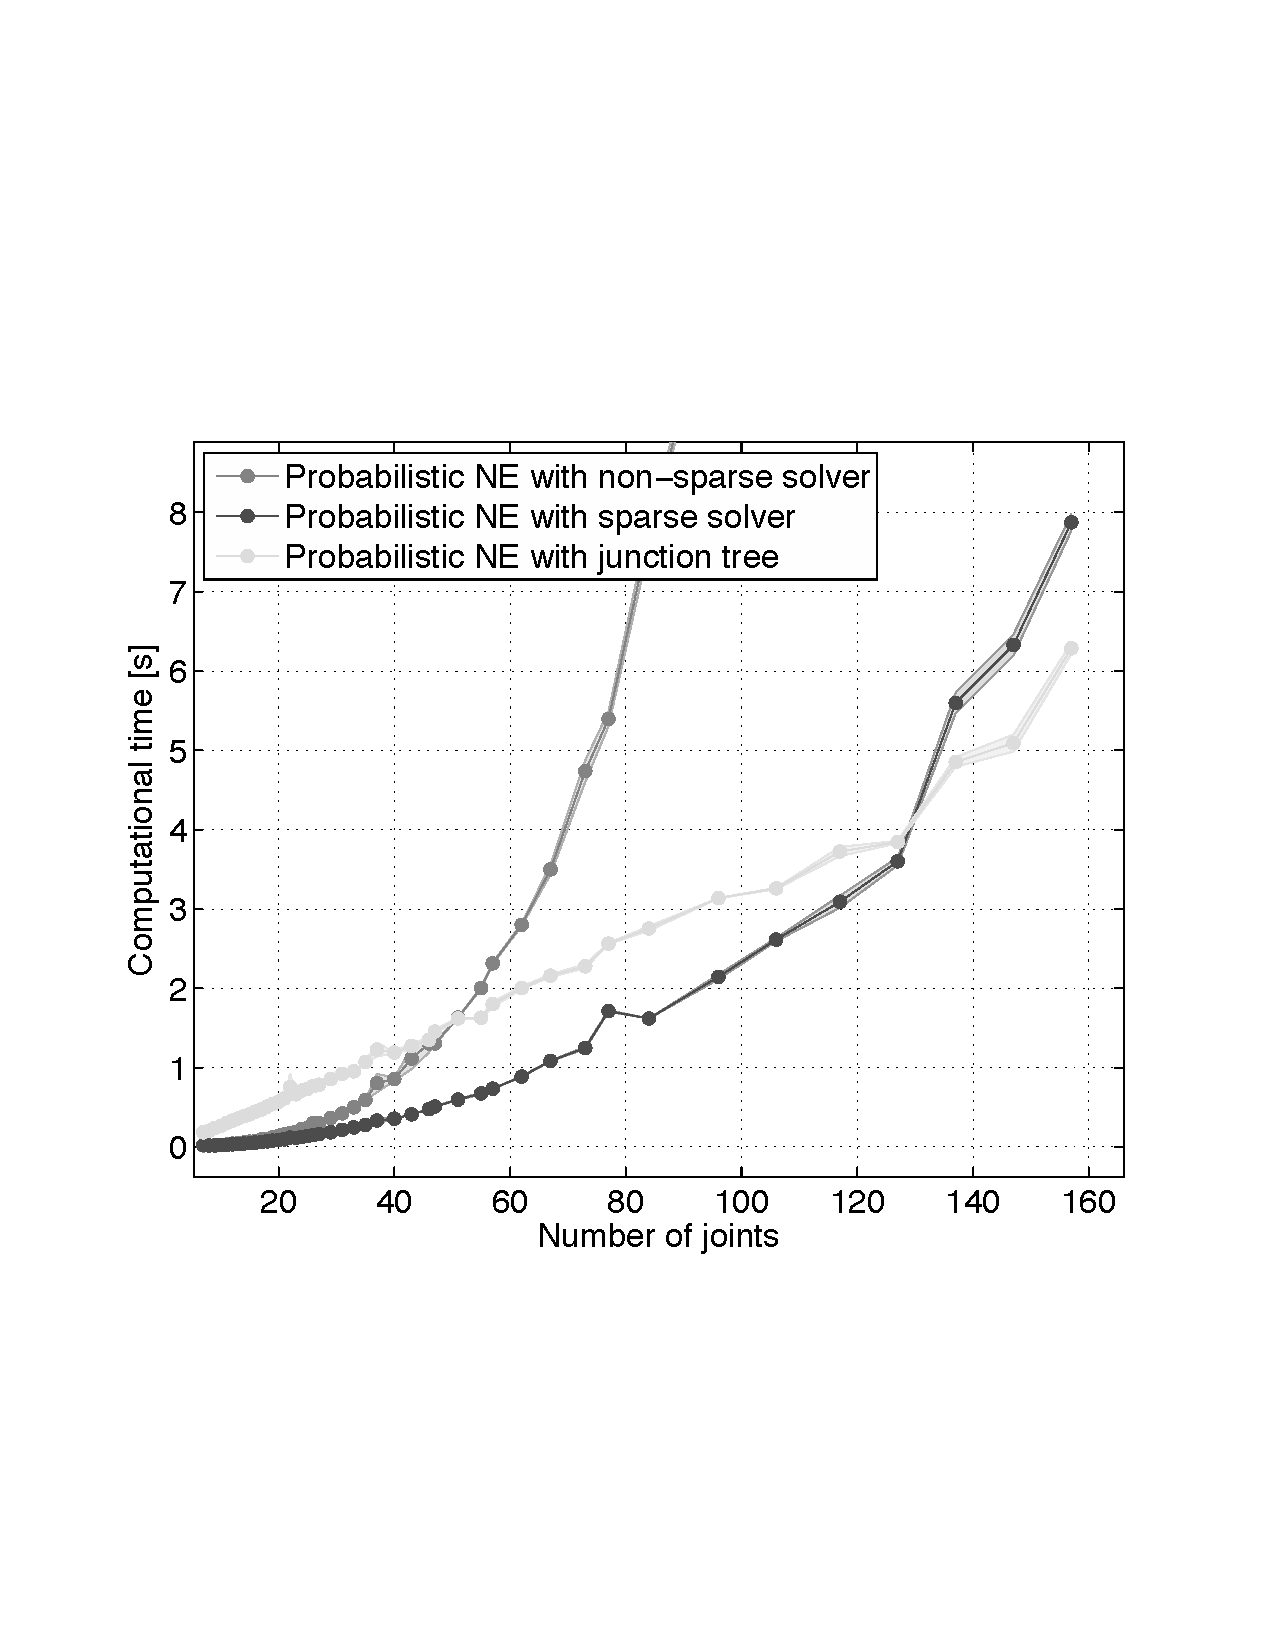
\includegraphics[height=0.35\hsize]{images/varTimeComplete.pdf} 
\caption{\label{fig:varTimeComplete} Comparison of non-sparse (S1-gray), sparse (S2-dark-gray) and Bayesian network junction tree (S3-light-gray) solvers in solving maximum-a-posteriori dynamics with redundant measurements (see \cite{Nori2015} for details).}
\end{figure}

\begin{figure*} [!ht]
  \centering 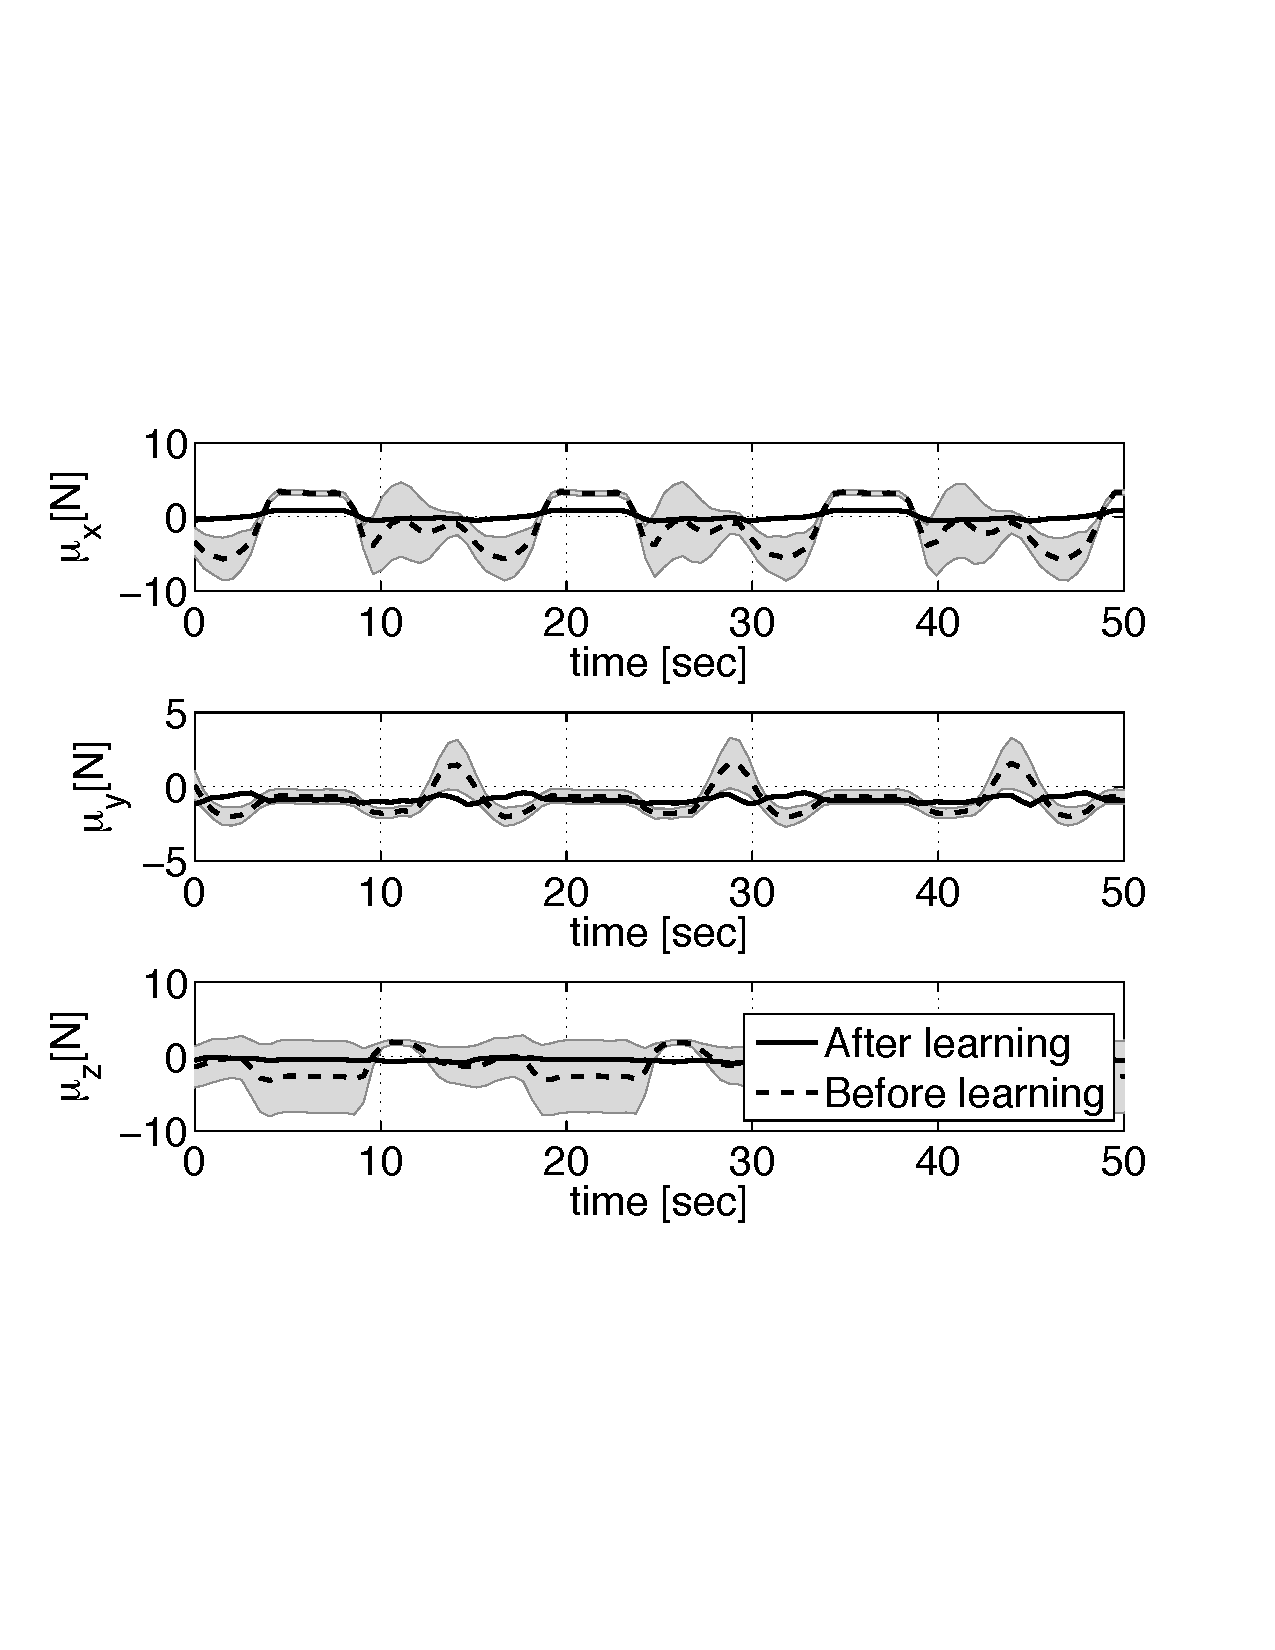
\includegraphics[width=0.45\hsize]{images/torques.pdf}  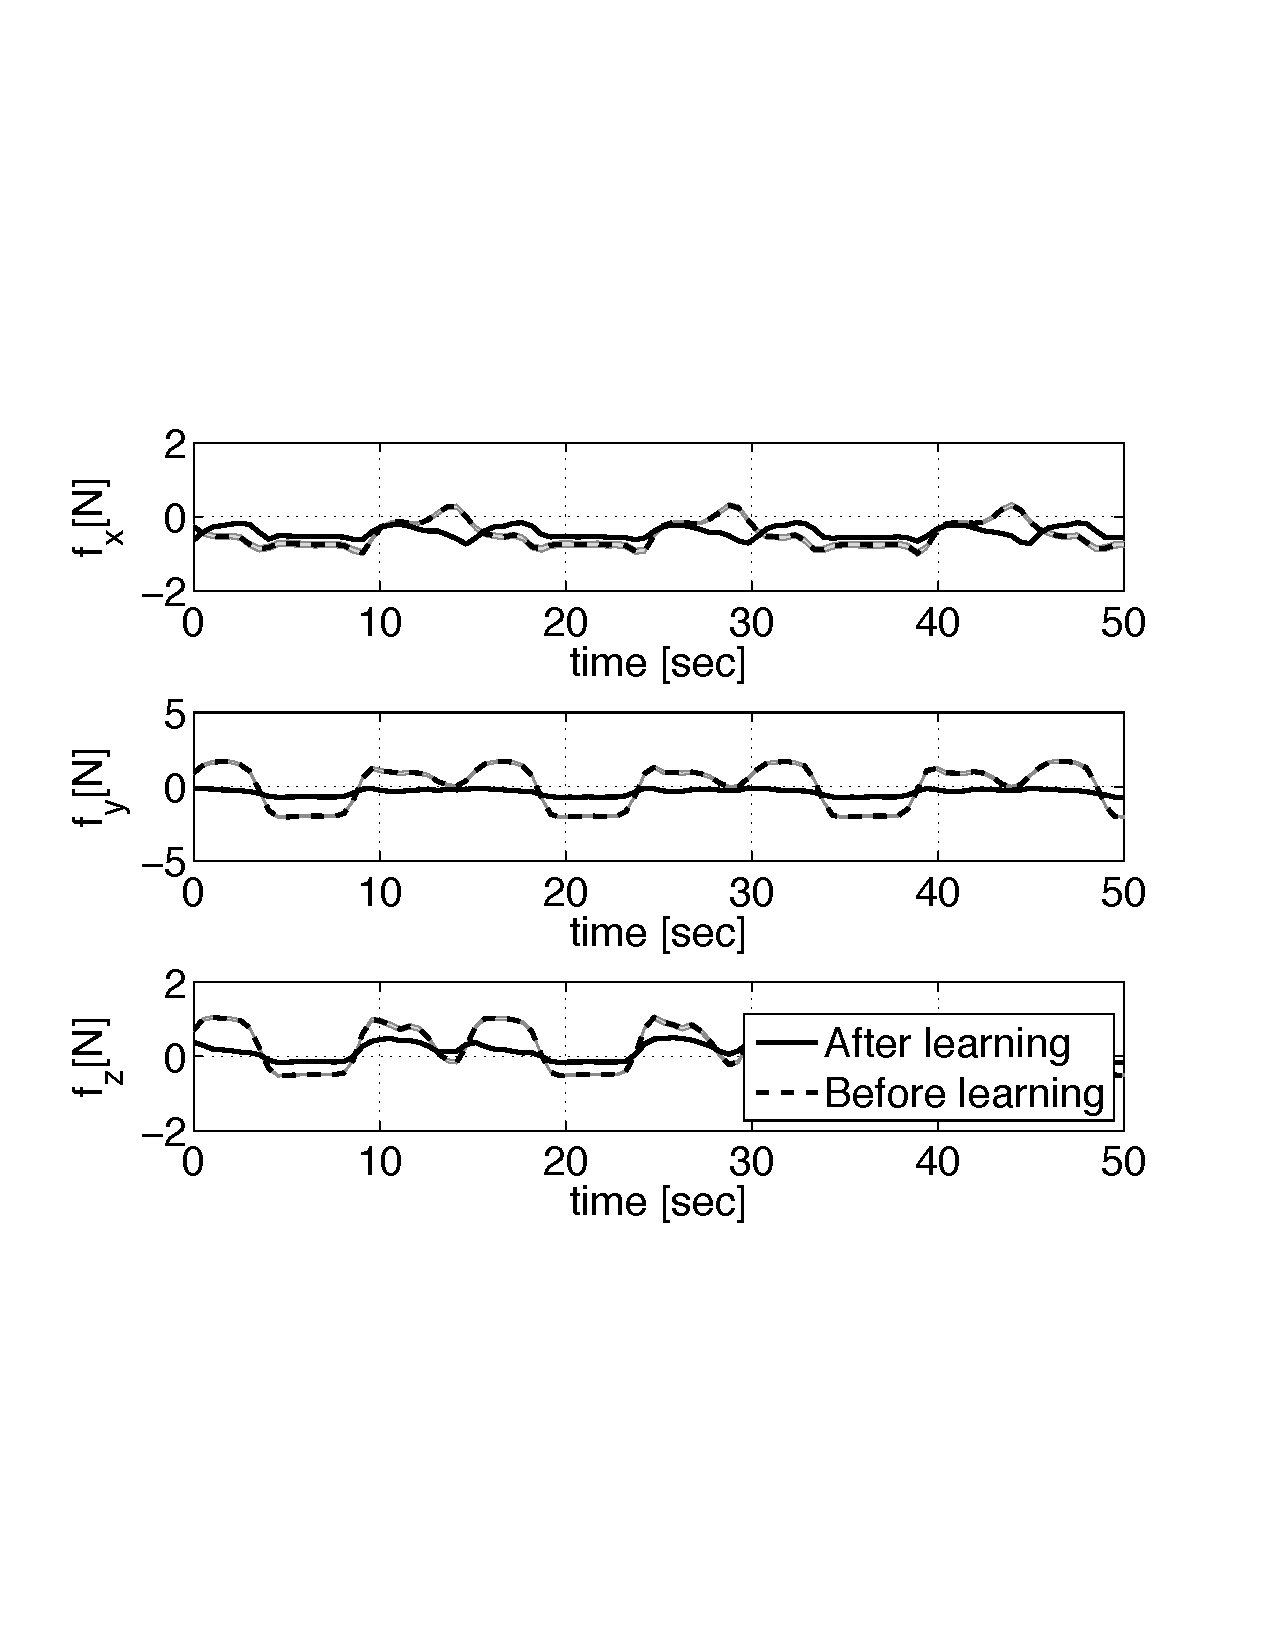
\includegraphics[width=0.45\hsize]{images/forces.pdf} 
\caption{\label{fig:extForceEstimation} The picture shows the errors in estimating an external wrench. The two curves refer to the estimation obtained before (dashed line) and after (solid line) the estimation of the data covariance with a modified EM algorithm \cite{Nori2015b}.}
\end{figure*}











